\section{Background}
In this section, we introduce some background knowledge about the low-rate TCP attack and SDN.

\subsection{The Low-rate TCP Attack}
The low-rate TCP attack consists of periodically pulsing flows which has an impact on benign TCP flows. The periodic square wave is a typical form of the attack \cite{b20}. We denote the link capacity of a switch as $C$, the period of the attack as $T$, and the burst length of the square wave as $L$ units of time within each period. We denote the ratio $L / T$ by $\eta$. During the burst, the square wave has a peak rate of $R$. We can calculate that the average rate of this form of attack is $\eta \cdot R$. During the burst of the attack traffic, the victim switches will be filled up with attack packets, which result in high packet loss of benign TCP flows. Thus, TCP flows are forced to continuously retransmit. Note that $\eta$ should be small to avoid being detected due to high traffic rate.

Figure~\ref{fig:LDoS} illustrates the attack traffic that can be described by three parameters ($R, L, T$). Note that either a single host or multiple distributed hosts can generate low-rate TCP attack traffic \cite{b4}. Two approaches for generating a distributed attack are mentioned in \cite{b3}. Assuming that $D$ distributed hosts generate low-rate TCP attack, one method is to  generate the attack flows with the same period $T$ and the burst rate $R/D$. Another method is to generate attack flows with the period $DT$ and the burst rate $R$. The low-rate TCP attack traffic is distributed in different attack sources and needs to be synchronized so that the aggregate traffic forms the desired square wave at the targeted link. 

\begin{figure}
\vspace{-0.2in}
\centering
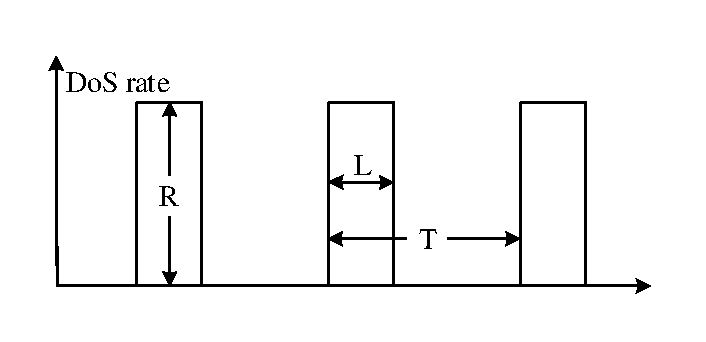
\includegraphics[width=3.4in]{Design/LDoS.pdf}
\vspace{-0.1in}
\caption{\small{Low-rate TCP attack traffic.}}
\label{fig:LDoS}
\vspace{-0.2in}
\end{figure}



\subsection{Counters and Meters of SDN}
In SDN, \emph{counters} are enabled to collect the information of the switches. They can help the controller to detect the low-rate TCP attack and locate the hosts. Counters can be obtained from the flow rules and the switches' port. In a switch, packets are matched by the flow rules and the highest priority flow rule that matches the packet will be selected to deal with the packet. The counters associated with the flow rule will be updated. Moreover, if the packet is transmitted by a port, the counter associated with the port will be updated. Counters can be used to monitor the throughput of flows. The counters associated with a flow rule matching all the TCP packets are used to collect statistics of the TCP flows in a switch. The counters associated with ports will help to detect the affected ports. The counters associated with forwarding rules will help to locate attack hosts. Considering that we have a sequence of the byte count $B$ with the sampling period $T_b$, the rate signals $R$ of a counter can be obtained by:

\vspace{-0.05in}
\begin{equation}\label{eq:sampling}
\ R_i=\frac{B_i - B_{i - 1}}{T_b}
\end{equation}

\textit{Meters} enable the SDN to implement rate limiting for flows and ports. The meter controls the rate of the aggregate of all flow rules to which it is attached. Note that, the \emph{burst\_size} defines the granularity of the meter. 
%To mitigate the low-rate TCP attack, the fine-grained meter is required for the low average rate of the attack.
